%% LyX 2.1.3 created this file.  For more info, see http://www.lyx.org/.
%% Do not edit unless you really know what you are doing.
\documentclass[twocolumn,english,10pt,conference,letterpaper]{RWWTemplate}
\usepackage[T1]{fontenc}
\usepackage{amsmath}
\usepackage{amssymb}
\usepackage{graphicx}

\makeatletter

\makeatletter

%%%%%%%%%%%%%%%%%%%%%%%%%%%%%% LyX specific LaTeX commands.
\special{papersize=\the\paperwidth,\the\paperheight}


%%%%%%%%%%%%%%%%%%%%%%%%%%%%%% User specified LaTeX commands.
\usepackage [nospace]{cite}

\@ifundefined{showcaptionsetup}{}{%
 \PassOptionsToPackage{caption=false}{subfig}}
\usepackage{subfig}
\makeatother

\usepackage{babel}
\begin{document}

\title{Maximum Likelihood Decoding for Non-Synchronized UHF RFID Tags }


\author{Hamed Salah, Hazem A. Ahmed, Joerg Robert, Albert Heuberger \\
Friedrich-Alexander-Universit�t Erlangen-N�rnberg (FAU)\\
\{hamed.kenawy, hazem.a.elsaid, joerg.robert, albert.heuberger\}@fau.de}
\maketitle
\begin{abstract}
In Radio Frequency Identification (RFID) systems, when multiple tags
reply at the same slot, collision occurs. The tags reply are with
different data and also different rates. The rate tolerance between
the tags reply reaches to +/-22\% of the nominal value of the rate
which plays a significant role for the stability and the efficiency
of RFID systems. This variation in the tags reply rates inhibit to
use the ML receiver which is very sensitive to the rate variation
between collided replies. This paper focuses on decoding the collided
tags with different rates in the RFID systems using Maximum Likelihood
(ML) receiver. A new algorithm is proposed to make the ML receiver
is insensitive the rate tolerance between the tags reply. The simulations
show that the dual receive antennas ML receiver that is used to recover
two collided tags over Rayleigh channel is not affected by the rate
tolerance. The receiver performance is compared with the previous
proposed dual antenna receivers, Minimum Mean Square Error (MMSE),
Zero Forcing (ZF), and Ordered SUccessive Cancellation (OSUC). The
proposed receiver outperforms the other types of receivers as it has
the largest diversity gain.
\end{abstract}


\section{Introduction}

Radio Frequency Identification (RFID) is an automatic identification
system that uses wireless communications to identify objects. Nowadays,
large amount of RFID tags are used in supply chain for product identification
\cite{Finkenzeller_book}, or sensor networks \cite{rfid_sensor_network},
where the cost and energy are critical. One of the biggest RFID challenges
is the capability to resolve collisions.

All the RFID tags are within the reading area of the reader are scheduled
using Frame Slotted Aloha (FSA). As a result of that, only a single
tag response can be decoded successfully, and in case of more than
single tag reply at the same slot, the collision occurs, therefore
the total slot will be discarded \cite{collision_def}. On the other
hand, the diversities of transmitted signals from different collided
tags, mainly on channel coefficient and data rates, may affect the
stability and efficiency of RFID system severely. In UHF RFID systems,
the data rate variations are much more crucial than in other communication
systems and if they are not taken into consideration, it would be
very difficult to make a correct decoding, leading to an inefficient
communication \cite{Synch_with_timing_recovery}. These data rate
variations appear from two factors that can not be mitigated in practical
systems. Firstly, due to low cost, RFID tags use a slow system clock
for the digital base-band operation, resulting in a measurement error
for the parameters that are transmitted by the reader to determine
the tag data rate. In the EPCglobal Class-1 Gen-2 RFID protocol, this
tag reply rate is called Backscatter Link Frequency (BLF) \cite{standard}.
Secondly, the tag clock frequency is usually affected by manufacturing
process variations, which also contribute to the BLF variations. Based
on the standard, a maximum BLF tolerance of $\pm22\%$ is allowed
with a BLF range from $\unit[40]{kHz}$ to $\unit[640]{kHz}$ \cite{standard}.
However, most of previous researches that focus on collision recovery
for RFID system assume that the collided tags have the same BLF which
is not valid assumption anymore.

Different groups paid attention on slots with colliding RFID tag replies.
Angerer et al. \cite{RFID_Reader_Receivers_MIMO} proposed an algorithm
for channel estimation for two colliding tags to be encoperated with
single and multiple antennas techniques to separate the collided tags.
However, they did not take the tolerance in the BLF into account in
his simulation. Also he did not use the optimum receiver because of
BLF tolerance. Kimionis et al. \cite{Inventory_time_reduction} proposed
a collision recovery technique to separate two and three collided
tags based on the tag reply encoding scheme properties. The proposed
algorithm will completely fail, if the tolerance of the BLF is taken
into consideration. Kaitovic et al. \cite{smart_collision_recov}
proposed a channel estimation technique that could be used to separate
up to eight collided tags per slot. However, this technique is not
compatible with the EPCglobal Class-1 Gen-2 RFID protocol and also
the rate tolerance is not taken into consideration.

In this paper, we present a collision recovery technique based on
Maximum Likelihood (ML) receiver with taking into consideration the
BLF tolerance. The ML decoding is very sensitive to the rate tolerance
between the collided symbols, so the proposed algorithm is used to
mitigate this sensitivity. The collision recovery technique is tested
with two collided tags with different tolerance values as based on
\cite{RFID_Reader_Receivers_MIMO}, there is no channel estimation
technique compatible with the standard \cite{standard} for more than
two tags.



This paper is organized as follows. Section 2 explains the most important
basics of the EPCglobal standard. In Section 3, The proposed ML decoding
technique is presented. In Section 4, the simulation results are discussed.
Finally, the conclusion is drawn in Section 5.


\section{EPCglobal Class-1 Gen-2}

\begin{figure}
\subfloat[FM0 basis functions\label{fig:FM0-basis-functions}]{\noindent \protect\begin{centering}
\protect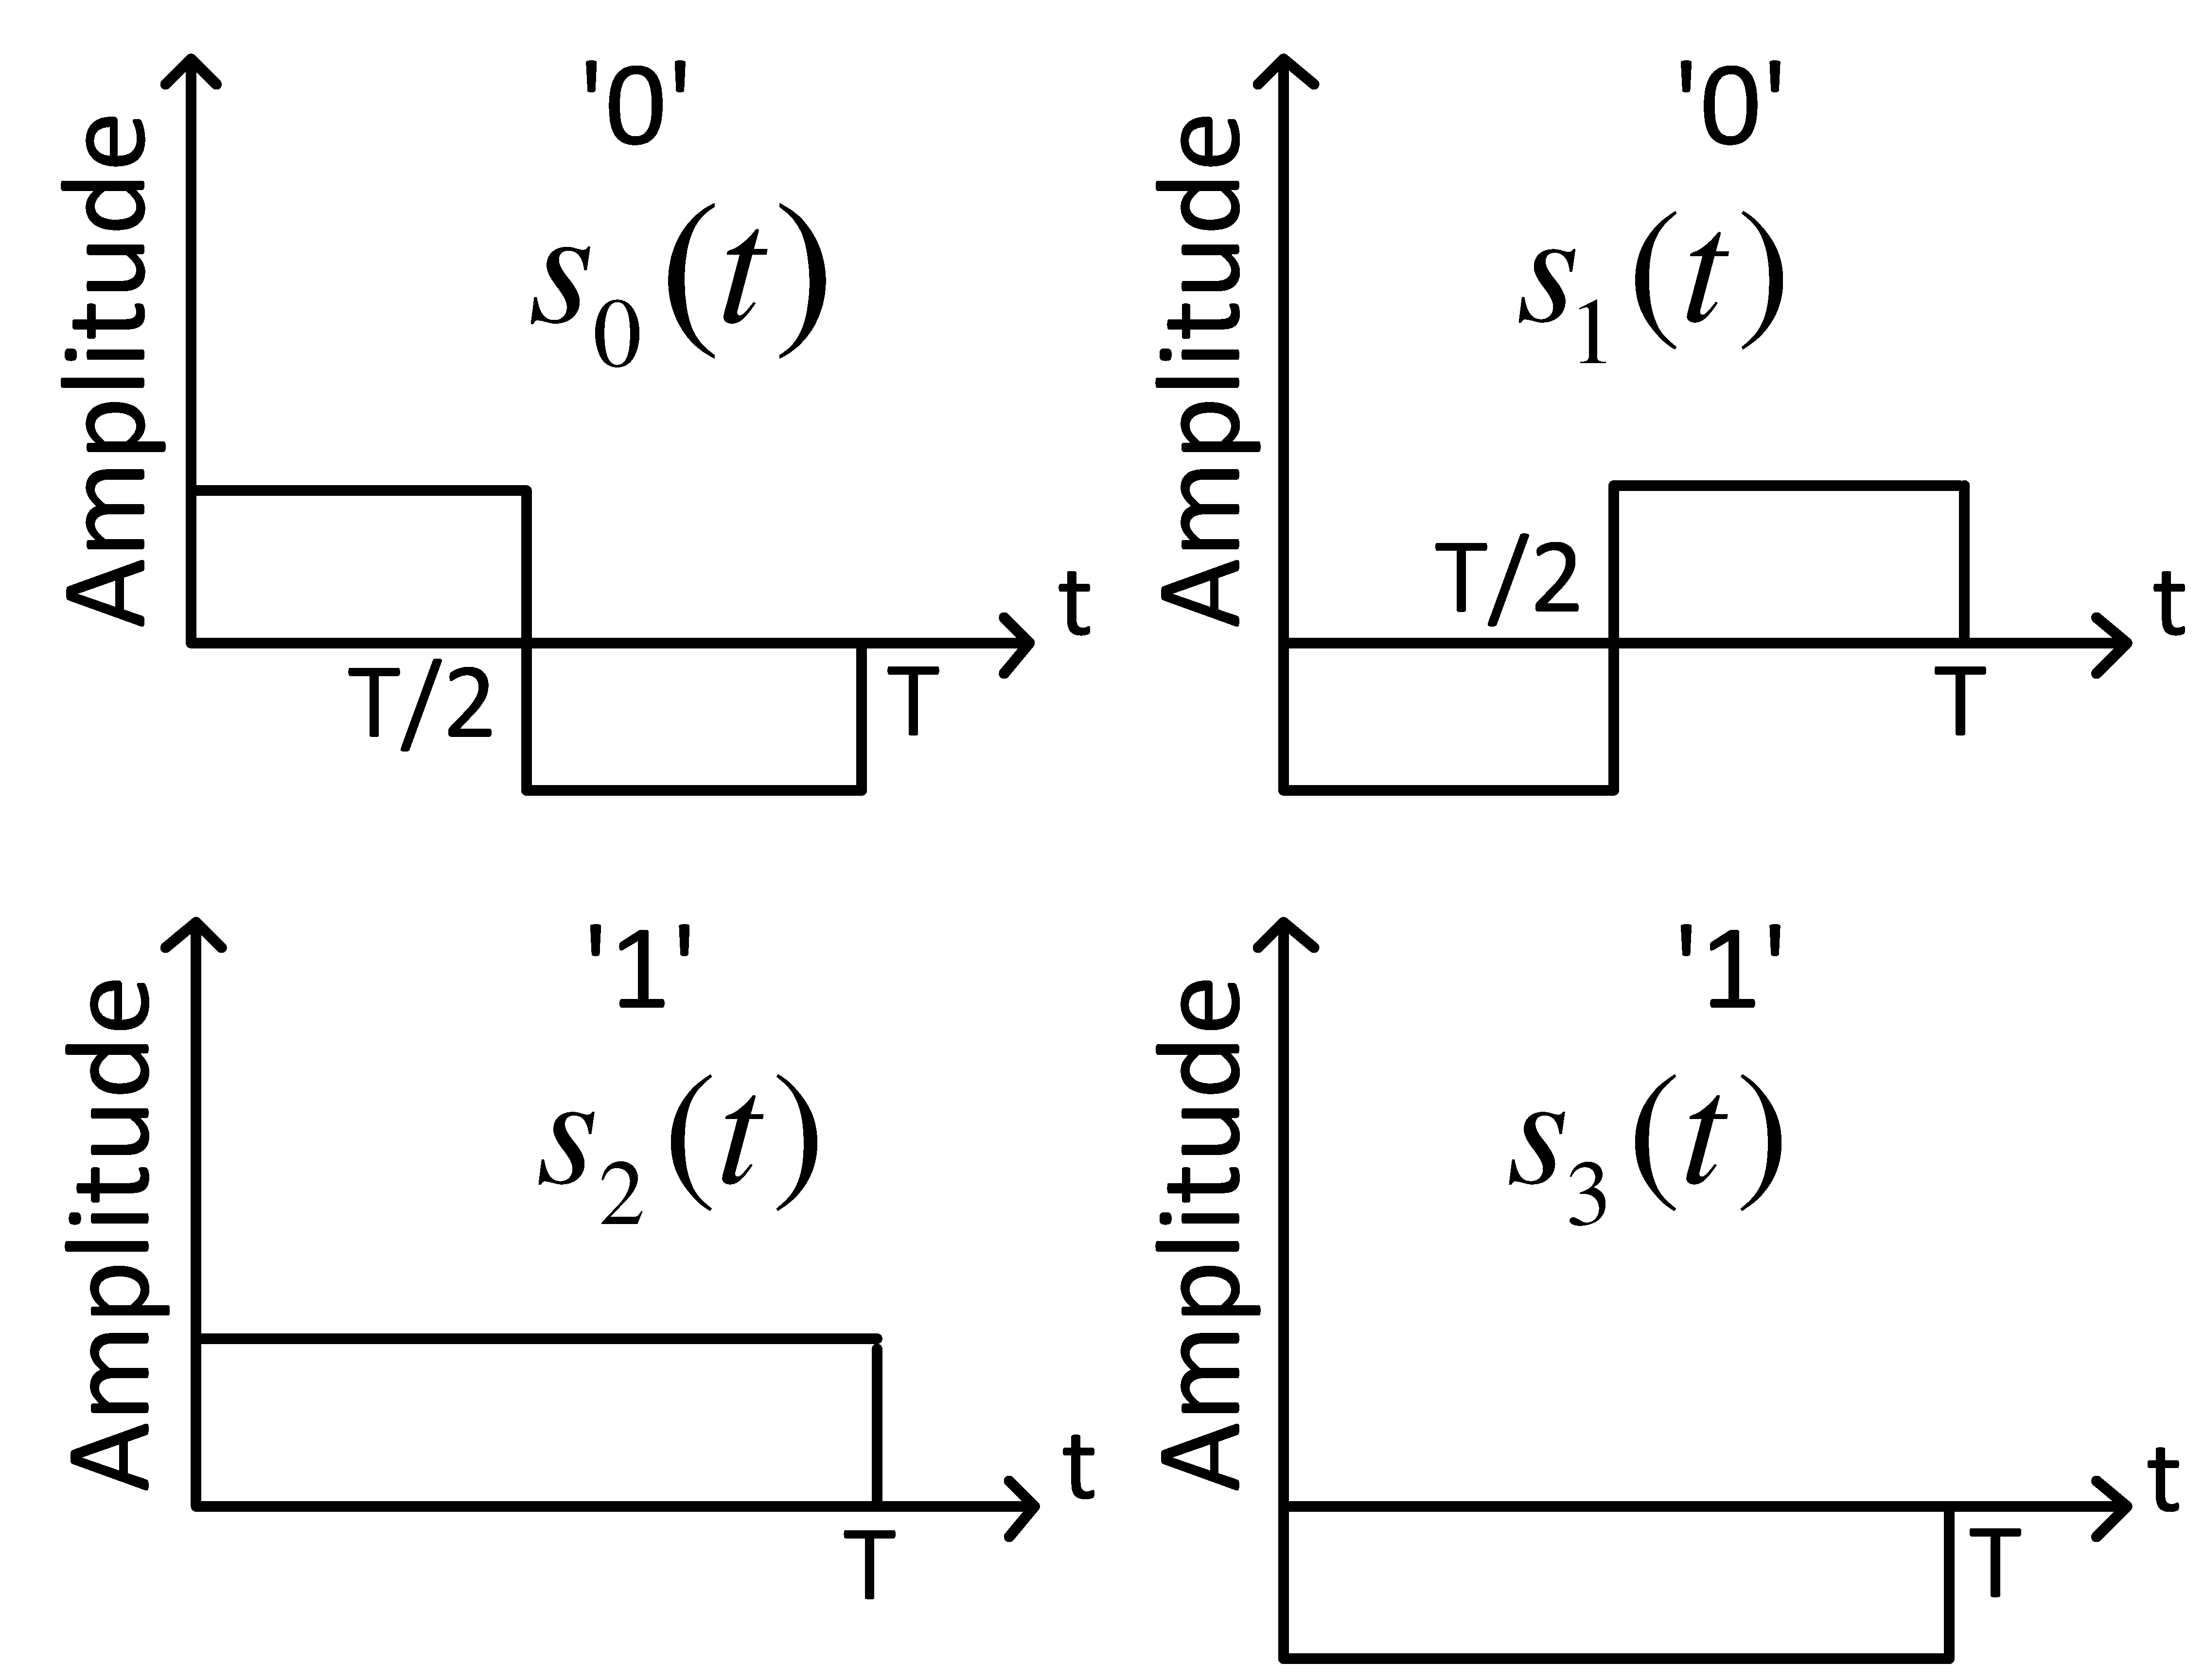
\includegraphics[scale=0.065]{FM0_waveform}\protect
\par\end{centering}



}\subfloat[FM0 sequences\label{fig:FM0-sequences}]{\noindent \protect\begin{centering}
\protect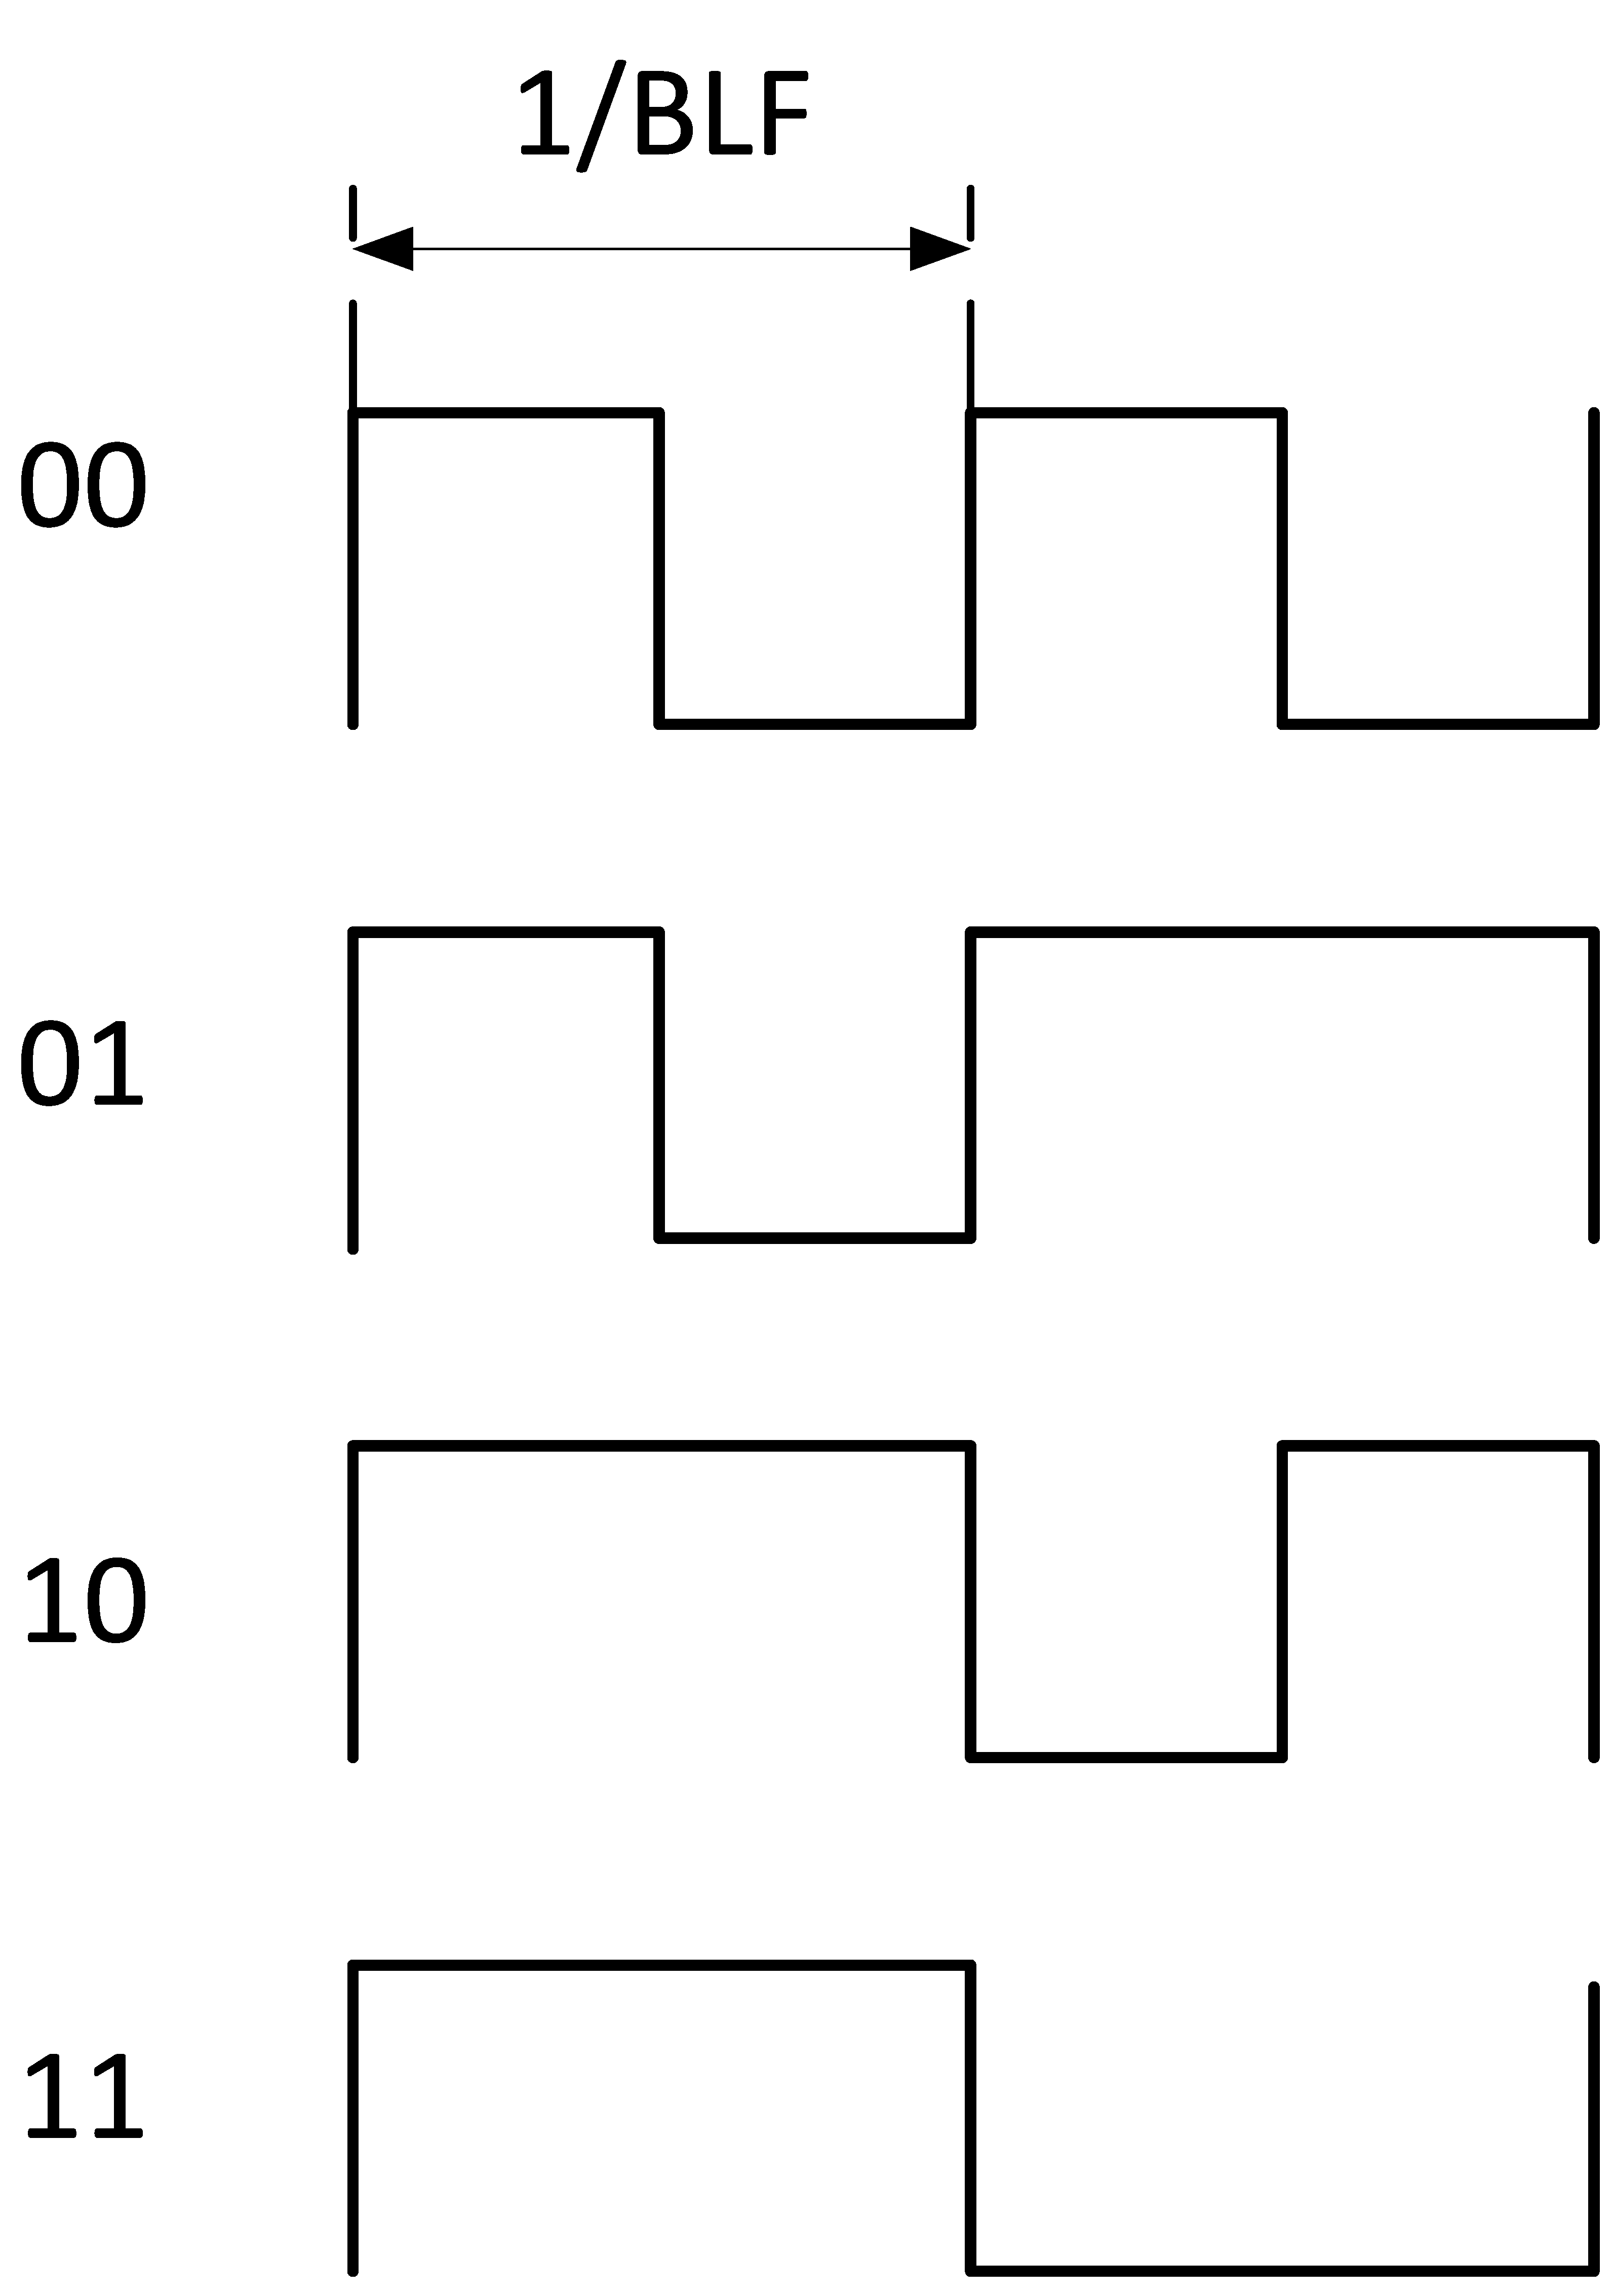
\includegraphics[scale=0.065]{FM0_waveform_ex}\protect
\par\end{centering}



}

\noindent \centering{}\protect\caption{FM0 encoding scheme \label{fig:FM0-Encoding}}
\end{figure}


According to the EPCglobal standard \cite{standard}, the tag uses
either FM0 (bi-phase space) or Miller to encode its data. As the FM0
encoding offers the higher data rate, most of the readers use this
encoding scheme and this paper focuses on it. The basis functions
$s_{n}(t)$ follow an FM0 (bi-phase space). In FM0 encoding, the pulse
shapes $s_{n}(t)$ for the symbols are selected among four pulse shapes
as shown in figure \ref{fig:FM0-basis-functions}, where $s_{0}(t)$
and $s_{1}(t)$ represent data-0 and $s_{2}(t)$ and $s_{3}(t)$ represent
data-1. The symbols are arranged to feature a level transition at
each boundary. For example, the pulse $s_{0}(t)$ can only be followed
by $s_{0}(t)$ or $s_{2}(t)$, but not by the symbol $s_{1}(t)$ or
$s_{3}(t)$ to keep the feature of a level transition between symbols
as shown in figure \ref{fig:FM0-sequences}. 

According to the standard, the nominal symbol duration value depends
on the tag reply encoding technique. It is a multiple of the inverse
of the BLF. In case of FM0 encoding, the symbol period is related
to the BLF by: $T=1/BLF$ as shown in figure \ref{fig:FM0-sequences}.


\section{ML Decoding for Collided Tags}


\subsection{System Model}

Figure \ref{fig:system-model} shows the basic communication between
two tags and a RFID reader, equipped with $N_{R}$ receive antennas.
In passive RFID systems the communication is half-duplex. The reader
provides the RFID tags with energy in form of a continuous carrier
transmission. During this energy signal the reader sends some specific
commands to the tags to tell them about the rate they should reply
with, the modulation technique that should be used, and the number
of available slots. Then the tags use the reader information to backscatter
their IDs. Because of this type of communication link, the channel
that each tag reply faces is a backscatter channel. The backscatter
channel is a forward channel (reader to tag) and a backward channel
(tag to reader) multiplied to each other. In \cite{radio_link_budget},
the authors proposed a two-way Rician channel model for RFID scenarios
based on carried out channel measurements. They also showed that since
Rician factor strongly depends on the environment, a better fit to
the measurement data was achieved by applying a double Rayleigh distribution.
We can describe the system by equation (\ref{eq:signal model})

\begin{equation}
\mathbf{y}=\mathbf{H}\cdot\mathbf{x}+\mathbf{n}\label{eq:signal model}
\end{equation}


where $\mathbf{H}$ represents $N_{R}\times R$ channel matrix with
channel elements $h_{ij}=h_{j}^{f}\cdot h_{ij}^{b}$, $y$ is the
$N_{R}\times1$ complex valued received signal vector, $x$ denotes
$R\times1$ the modulation signal vector from tags, and $n$ is the
$N_{R}\times1$ AWGN at receive antennas. In this work, we assume
that the transmit and receive antennas of the reader are perfectly
isolated so there is no carrier leakage.

\begin{figure}
\noindent \begin{centering}
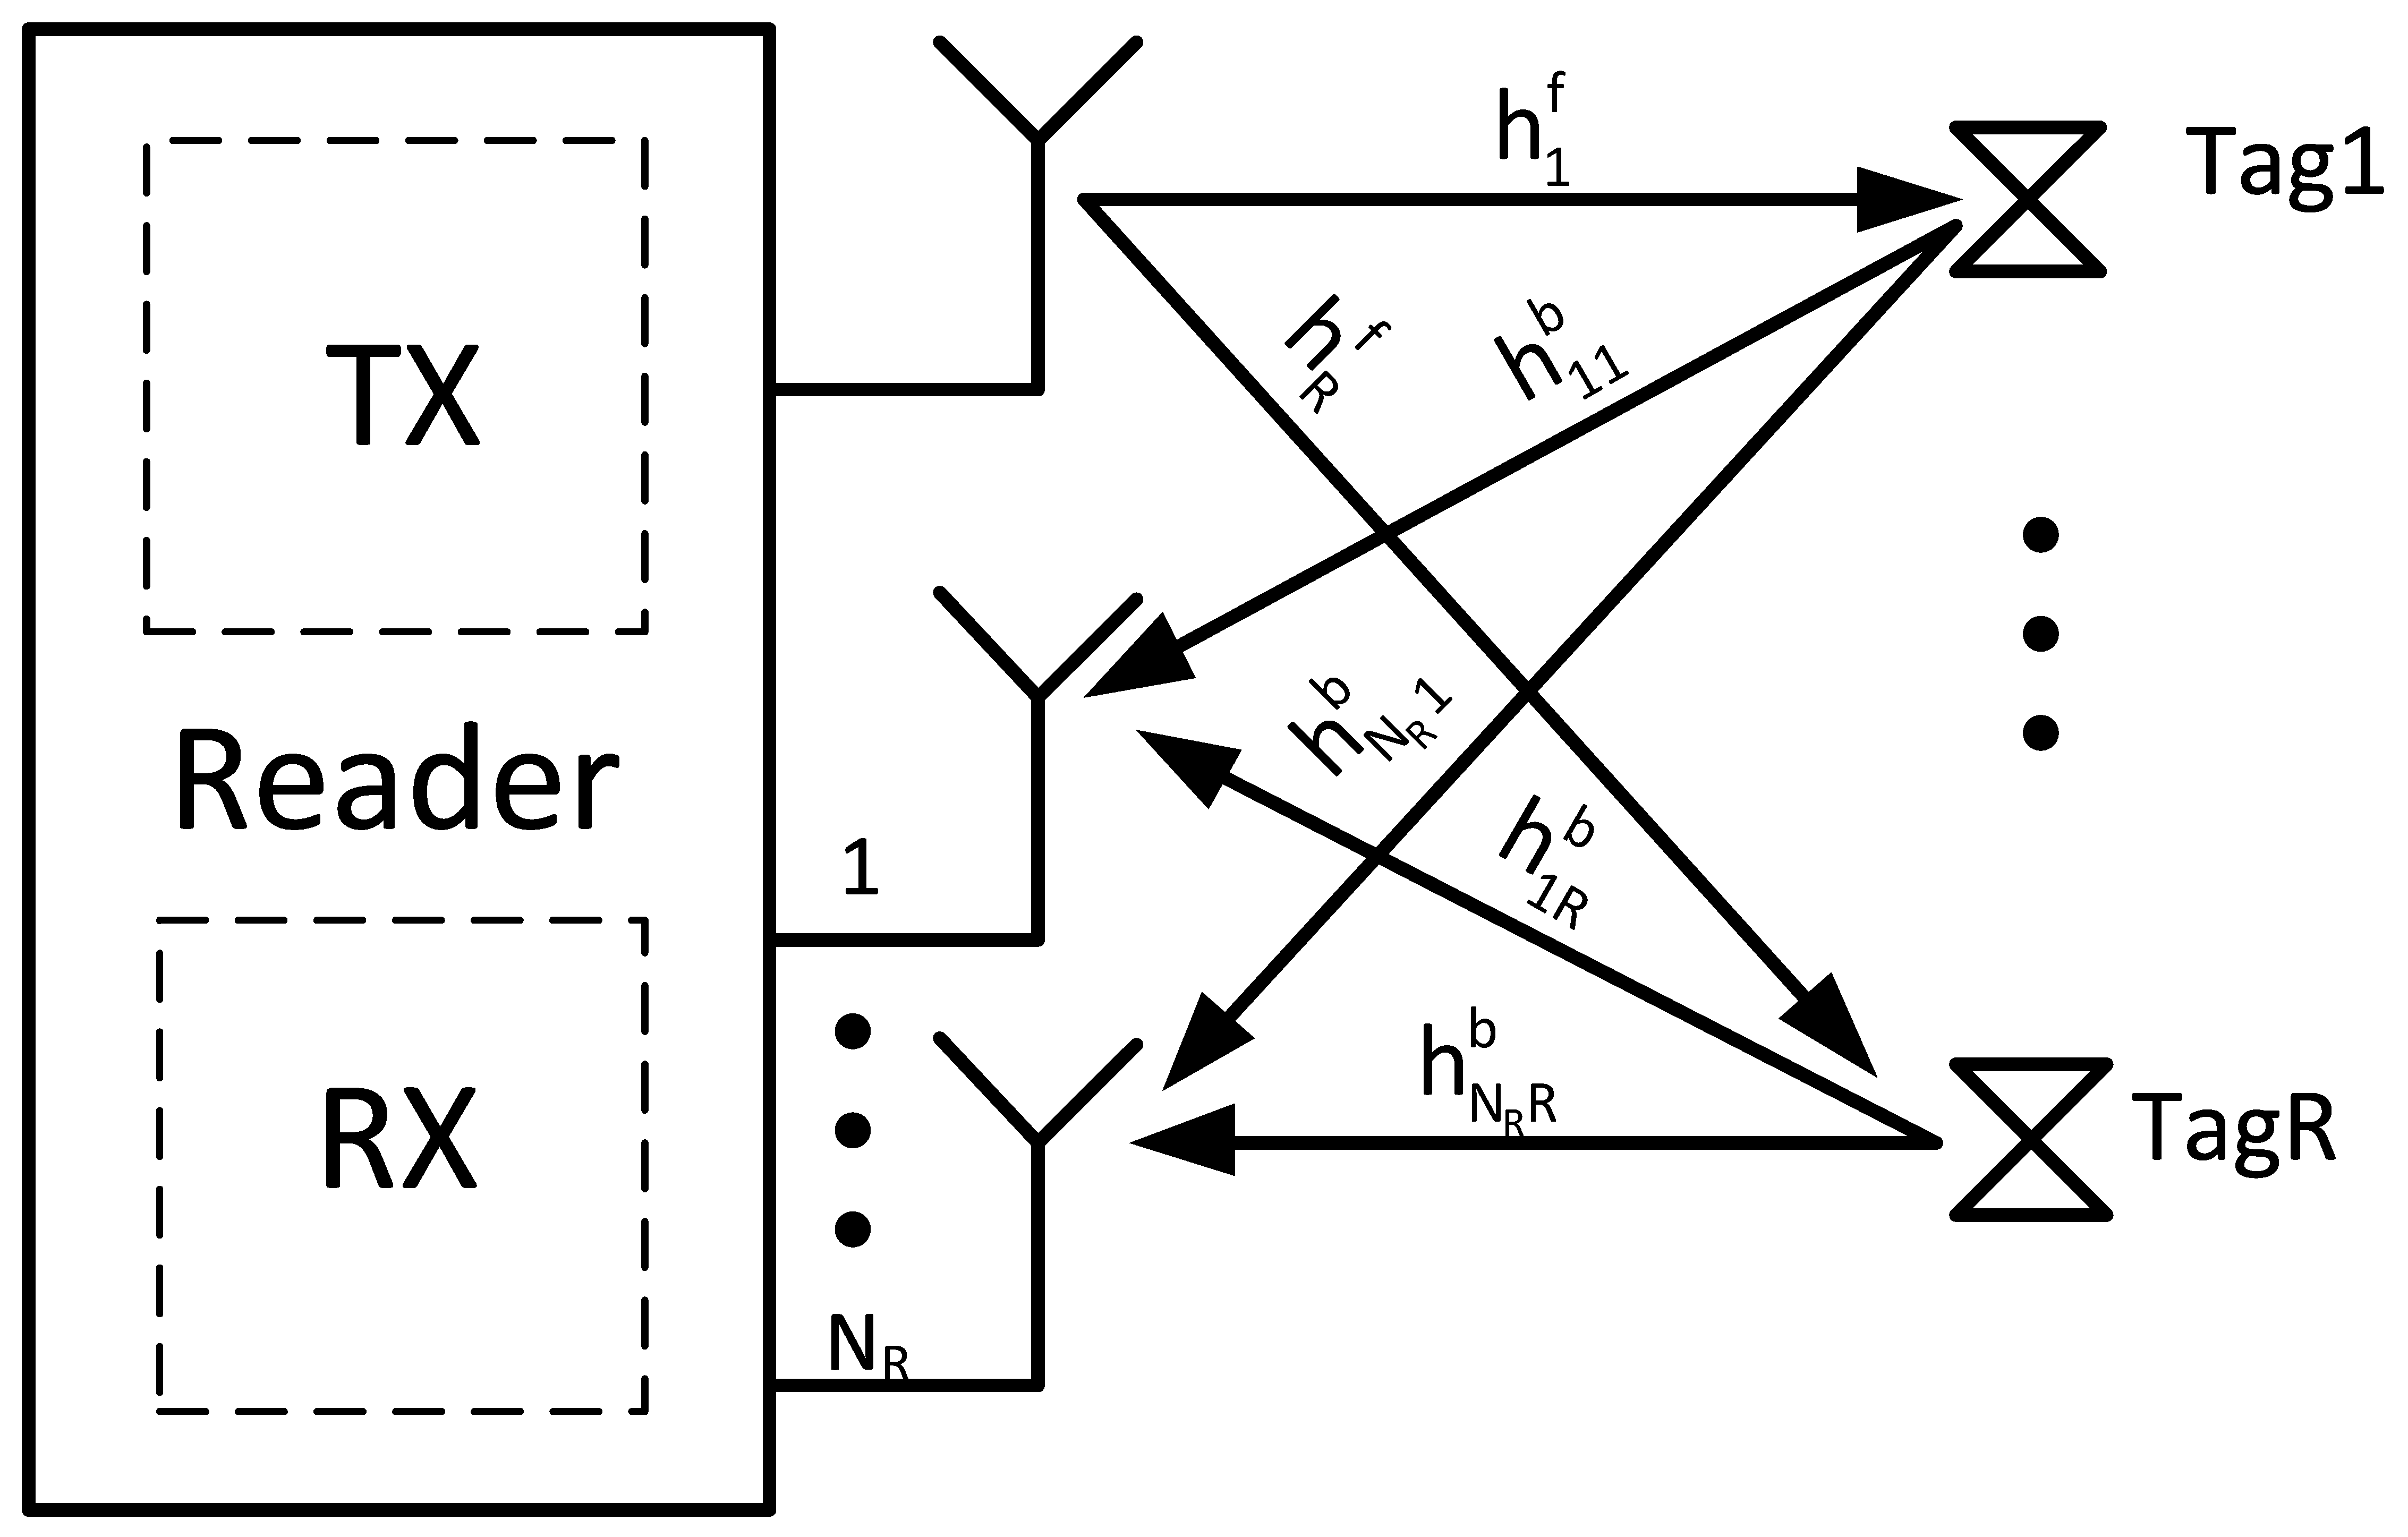
\includegraphics[scale=0.09]{system_model}
\par\end{centering}

\protect\caption{Communication between a reader and two tags\label{fig:system-model}}


\end{figure}



\subsection{ML Decoding for Non-Synchronized Collided Tags}

The objective of the receiver is to obtain an estimate of the modulation
signal of tags, $\mathbf{x}$, from the given received data in $\mathbf{y}$
over Additive White Gaussian Noise (AWGN) with noise variance $\sigma_{n}^{2}$,
through channel $\mathbf{H}$. There are a wide variety of techniques
for doing this but as stated in the introduction this work will only
be concerned with the maximum likelihood (ML) detector. The ML detector
has the desirable property that, it minimizes the probability of error,
\begin{equation}
P_{e}\triangleq P(\mathbf{x}\neq\hat{\mathbf{x}})\label{eq:prob. of error def}
\end{equation}


Minimizing the probability of error is equivalent to maximizing the
probability of correctly estimating $\mathbf{x}$, i.e. $P(\mathbf{x}=\hat{\mathbf{x}}\mid y,\mathbf{H})$.
To maximize the probability of correctly estimating we have to maximize
the probability density function of $\mathbf{y}$ given $\mathbf{x}$,
and $\mathbf{H}$, $P(\mathbf{y}\mid\mathbf{x},\mathbf{\mathbf{H}})$
\cite{Proakis}

\begin{equation}
P(\mathbf{y}\mid\mathbf{x},\mathbf{H})=\frac{1}{\pi^{N_{R}}\sigma_{n}^{2N_{R}}}exp\left(-\frac{1}{\sigma_{n}^{2}}\left\Vert y-\mathbf{H}\mathbf{x}\right\Vert ^{2}\right)\label{eq:max_likelihood_eqn}
\end{equation}


Equation (\ref{eq:max_likelihood_eqn}) is referred to as the ML criterion
and the detector given by
\begin{equation}
\hat{\mathbf{x}}=arg\,\,\underset{\mathbf{x}\in X}{max}\,P(y\mid\mathbf{x},\mathbf{H})=arg\,\,\underset{\mathbf{x}\in X}{min}\left\Vert y-\mathbf{H}\mathbf{x}\right\Vert ^{2}\label{eq:likelihood_crit_eqn}
\end{equation}


The ML detector is the optimum receiver from performance point of
view. However, the performance of the receiver is severely affected
with the non-synchronization of the received symbol which is the case
in the RFID system as shown figure \ref{fig:ML decoding for non-synchronized tags}.
In this paper we propose an algorithm that makes the ML receiver does
not care about the synchronization between received symbols. Figure
\ref{fig:ML decoding for non-synchronized tags} shows two collided
with two different symbol duration, $T_{1}$ and $T_{2}$where $T_{1}<T_{2}$,
and $T_{i}=\frac{1}{BLF_{i}}$. The problem of non-synchronized tags
is that the symbol of the tag that has a lower symbol duration $T_{1}$
overlaps two symbols of the tag that has an higher symbol duration
$T_{2}$. For example the second symbol of Tag1 overlaps the second
symbol of Tag2 in an interval equals to $T_{2}-2\delta$ and $\delta$
of the first symbol, where $\delta=T_{2}-T_{1}$. The overlap between
symbol $i$ of Tag1 and symbol $i$ of Tag2 equals to $T_{2}-i\text{\ensuremath{\cdot\delta}}$.
In addition to the overlap between symbol $i$ of Tag1 and symbol
$i-1$ of Tag2 equals to $\left(i-1\right)\text{\ensuremath{\cdot\delta}}$.
Based on the this formulation of the rate tolerance problem, we designed
an algorithm to solve the problem. First, we have assumed that $BLF_{1}$
and $BLF_{2}$ are accurately estimated using MUSIC algorithm \cite{raey}.
Then the generated vector $x$ will contain two elements as we are
taking two collided tags as an example. Assume we are talking about
decoding symbol $i$ of Tag1; the first element in vector $x$ will
be a symbol $i$ of Tag1 with symbol length $T_{1}$, and the second
element is $T_{2}-i\delta$ of symbol $i$ and $\left(i-1\right)\cdot\delta$
of symbol $i-1$. This process would be repeated till the end of Tag1
symbols, then the remaining part of Tag2 symbols can be decoded separately
as in this part there is no collision. The decision on Tag1 symbols
can be taken directly, but the symbols of Tag2 should be reconstructed
first and then decoded using regular correlator receiver.

\begin{figure}
\noindent \begin{centering}
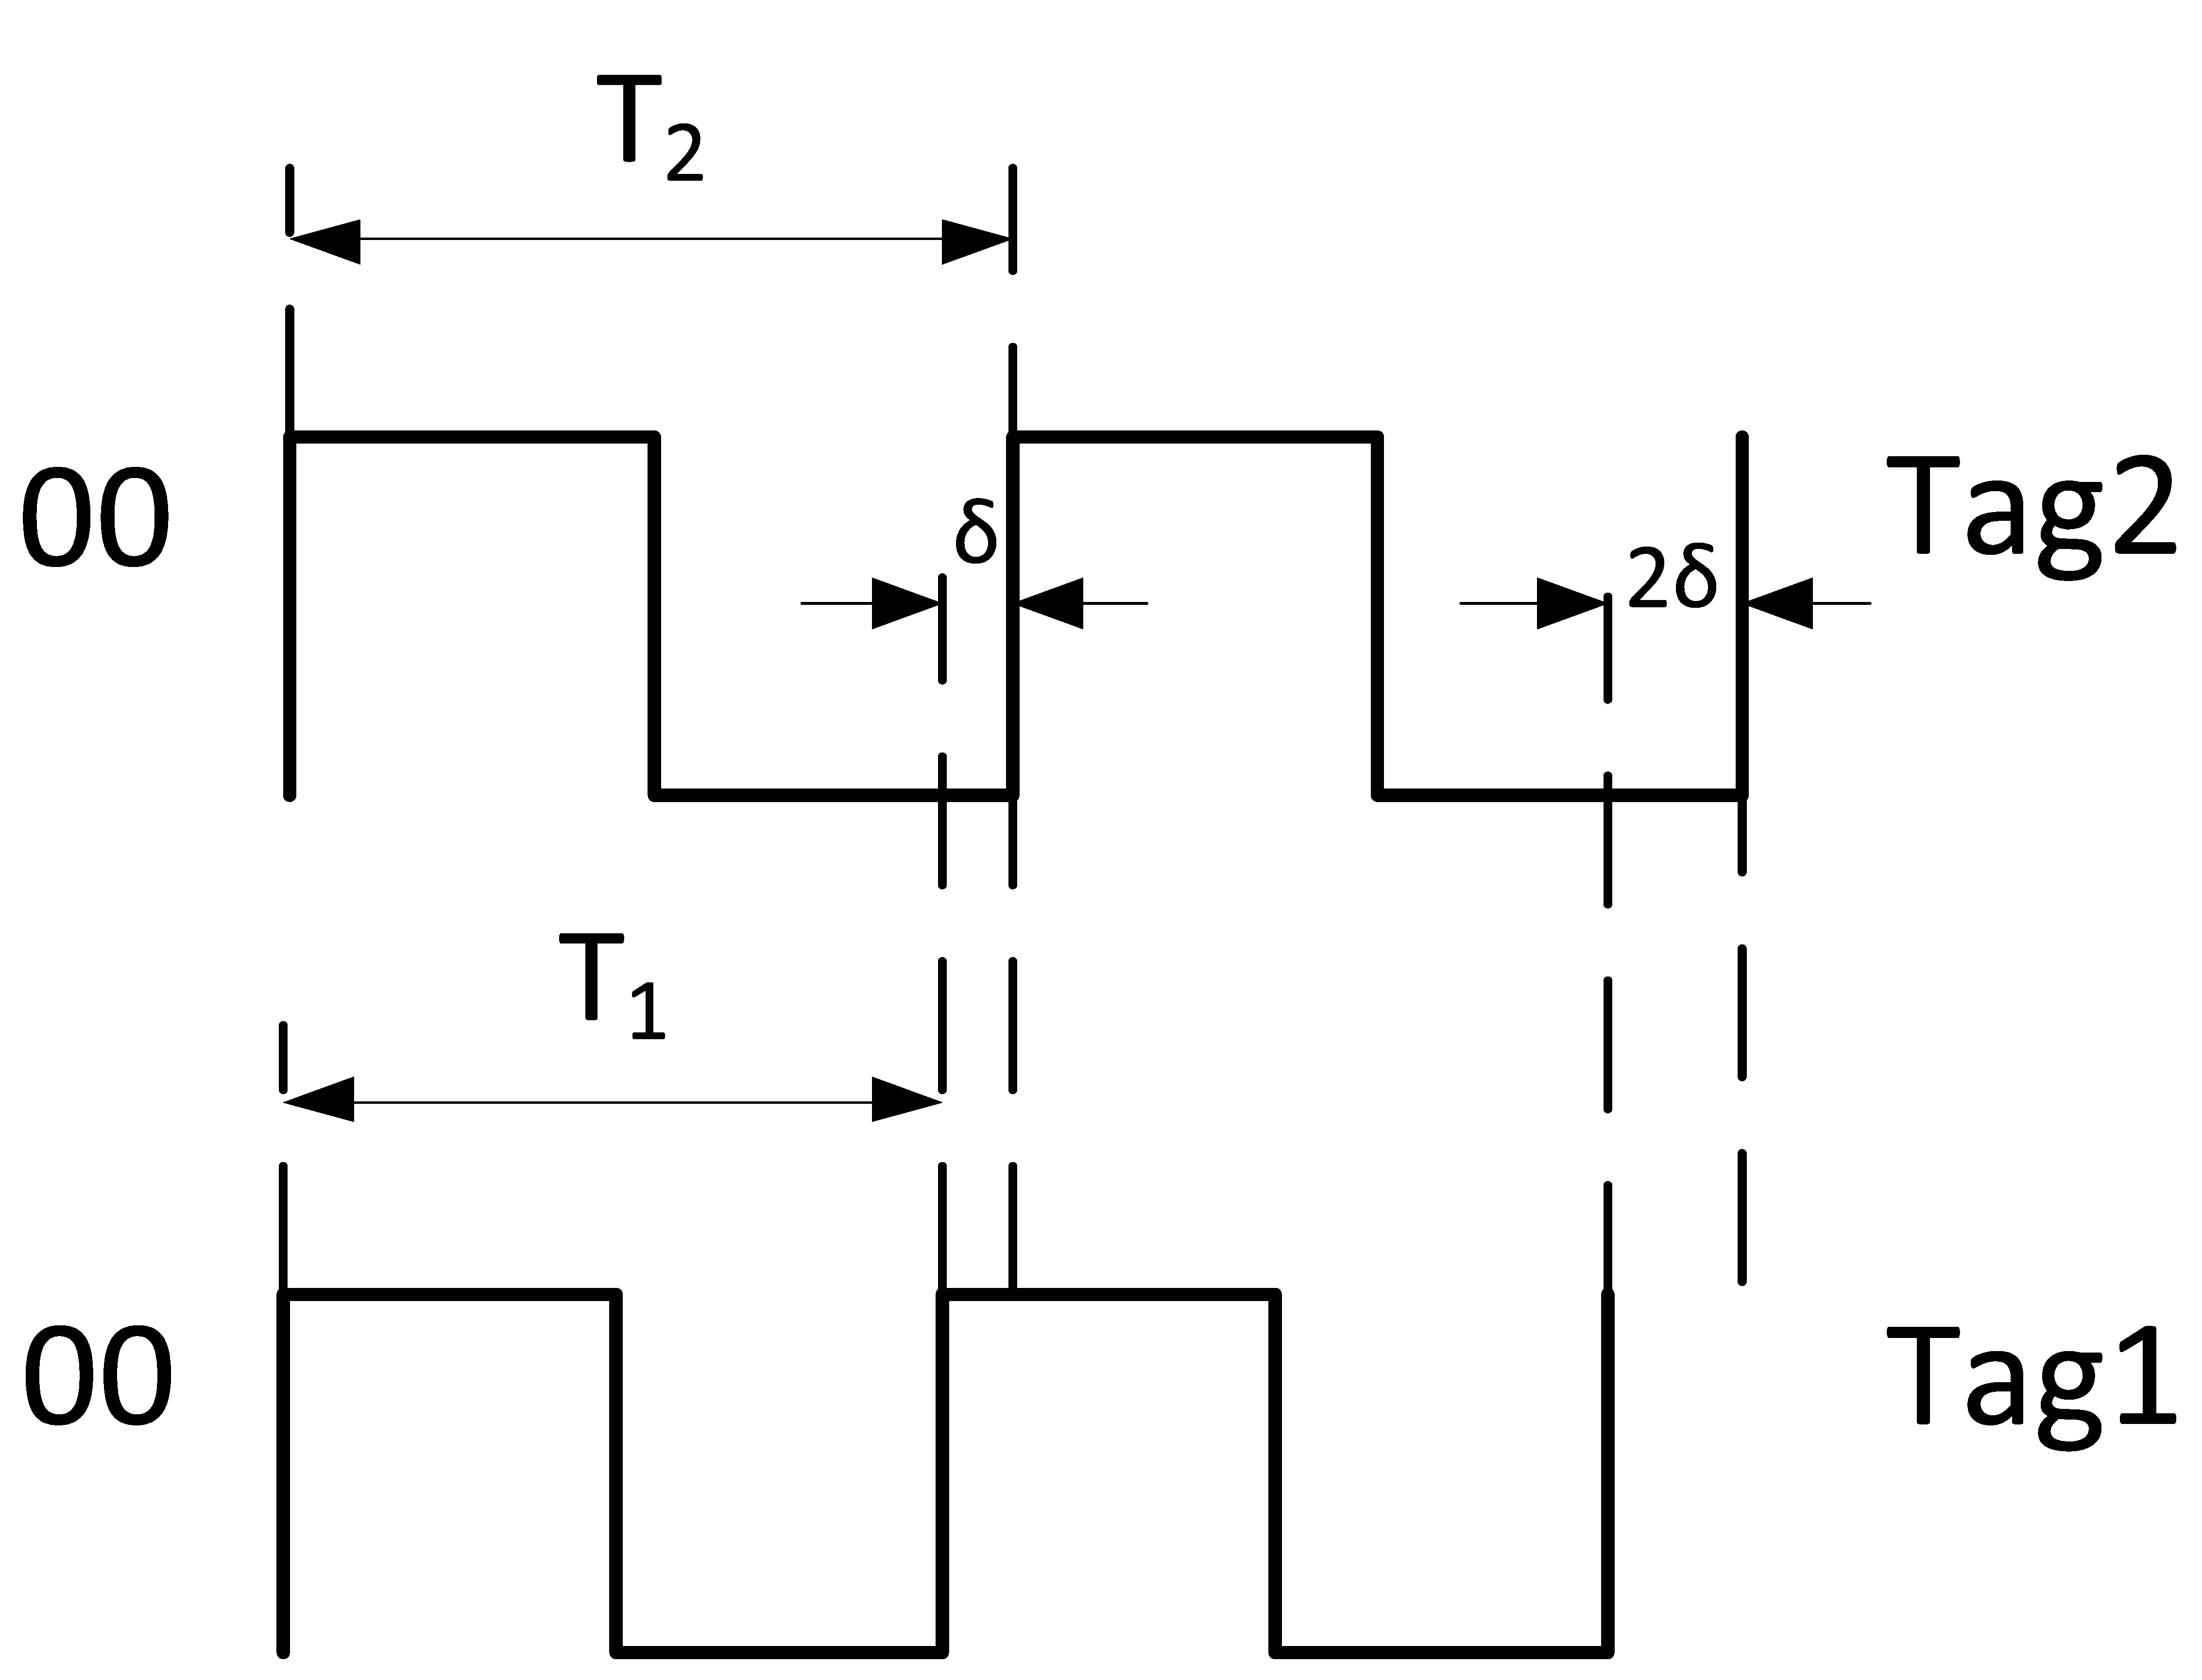
\includegraphics[scale=0.065]{non_sync_tags}
\par\end{centering}

\protect\caption{ML decoding for non-synchronized tags\label{fig:ML decoding for non-synchronized tags}}
\end{figure}



\section{Simulation Results}

For the sake of a simple comparison, we assume that the equivalent
channel matrix $\mathbf{H}$ follows a Rayleigh fading. The single
Rayleigh channel coefficient are independent zero mean circularly
symmetric complex Gaussian random variables with normalized energy
$E\{\left|h_{i}\right|^{2}\}=1$, which indicates the two collided
tags have the same average path loss. Figure \ref{fig:Bit-Error-Ratio rate tolerance }
shows the performance of the proposed ML receiver with dual antennas
when the tolerance in BLF equals to $0$, $5$, and $22\%$ and how
the performance is not affected by the value of tolerance. In the
simulation, both tags of uncoded random data are decoded depending
on the average received SNR $\gamma=\frac{1}{N_{R}}\sum_{j}\bar{\gamma}_{j}$,
where $\gamma_{j}=\left|h_{ij}\right|^{2}x_{i}^{2}/\sigma_{i}^{2}$
is the instantaneous SNR at antenna $j$ for tag $i$, and $\bar{\gamma}_{j}=E\{\gamma_{j}\}$.
Additionally to disturbance by noise, each stream is interfered by
the second tag responding in the same slot, with the same average
power. The channel coefficients are estimated by Angerer method \cite{RFID_Reader_Receivers_MIMO}.

\begin{figure}
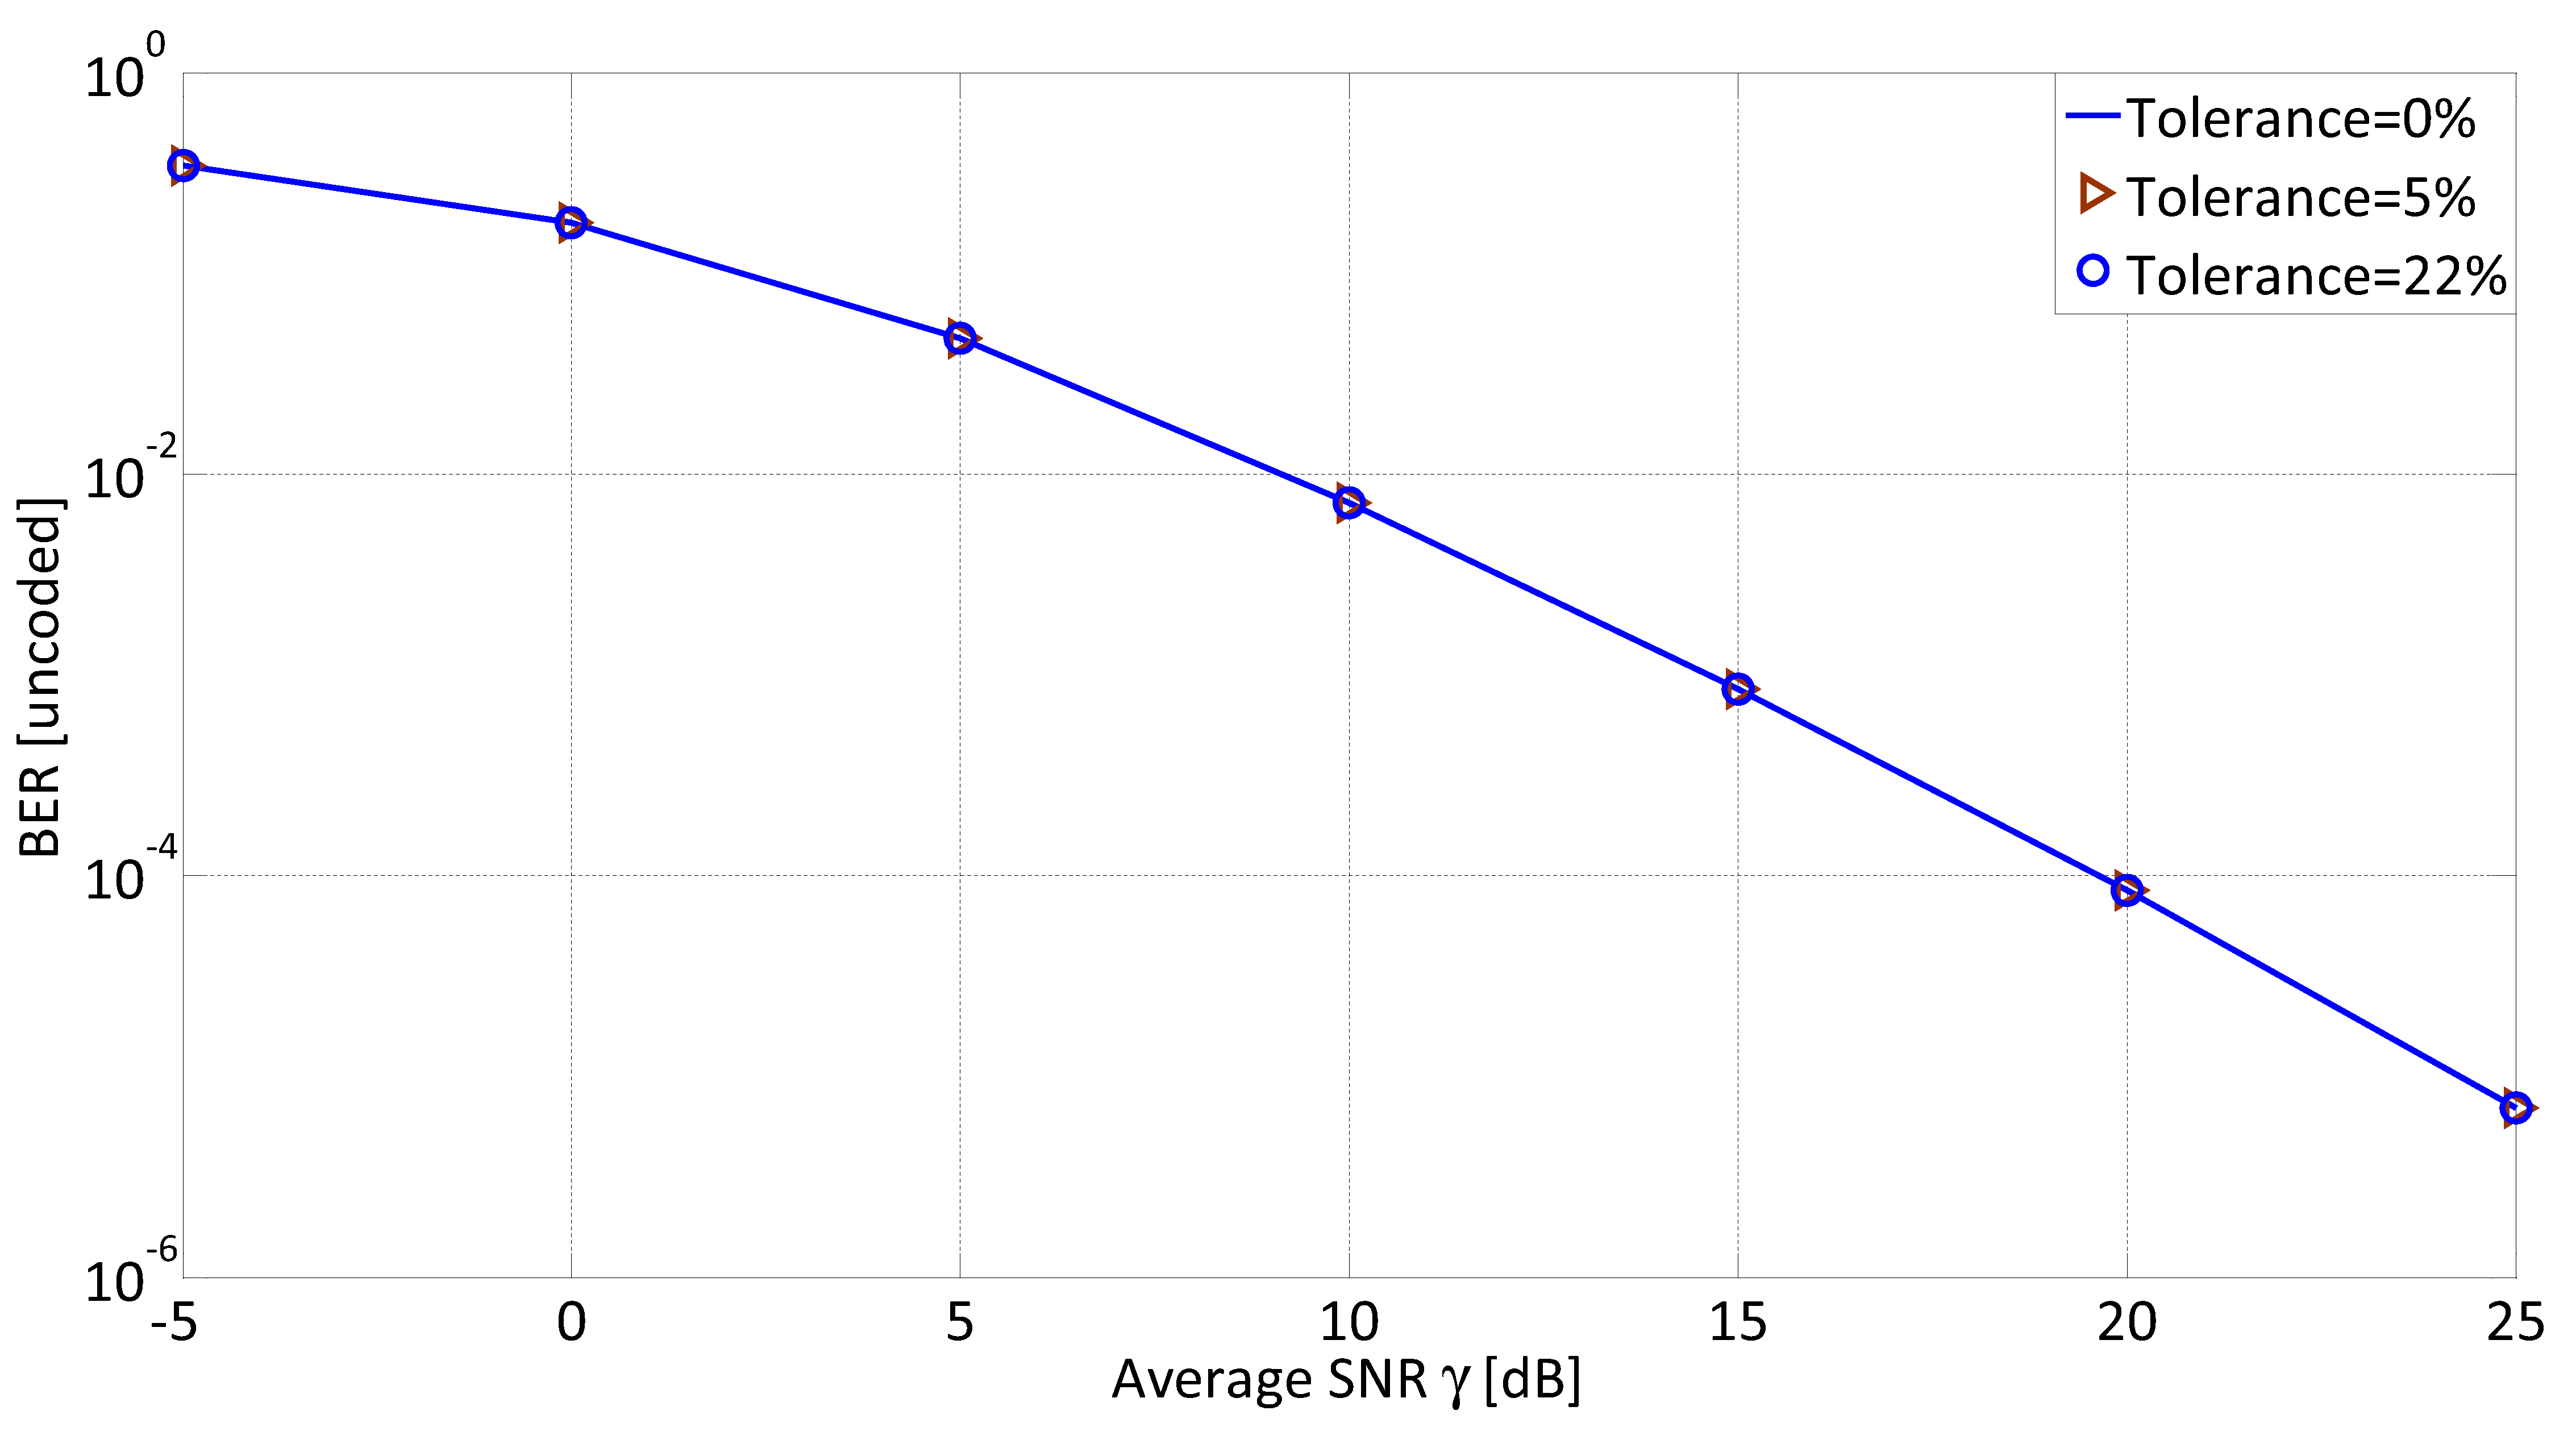
\includegraphics[scale=0.12]{BER_RayleighChannel_0_5_15Tolerance_modified}

\protect\caption{Bit Error Ratio for two receive antennas receiver in Rayleigh fading
channel in collision slots of two tags with $0$, $5$, and $22\%$
BLF tolerance \label{fig:Bit-Error-Ratio rate tolerance }}
\end{figure}


Figure \ref{fig:Bit-Error-Ratio-ML_MMSE-zf-OSUC} shows the performance
of various dual antenna receivers. As expected, the simple Zero Forcing
(ZF) receiver shows the worse performance than the Minimum Mean Square
Error (MMSE) and Ordered SUccessive Cancellation (OSUC) \cite{RFID_Reader_Receivers_MIMO}.
Furthermore, the proposed ML receiver outperform all other receivers
that are proposed by \cite{RFID_Reader_Receivers_MIMO} by at least
$\unit[3]{dB}$ and also that was expected as the ML decoding is the
optimum receiver.

\begin{figure}
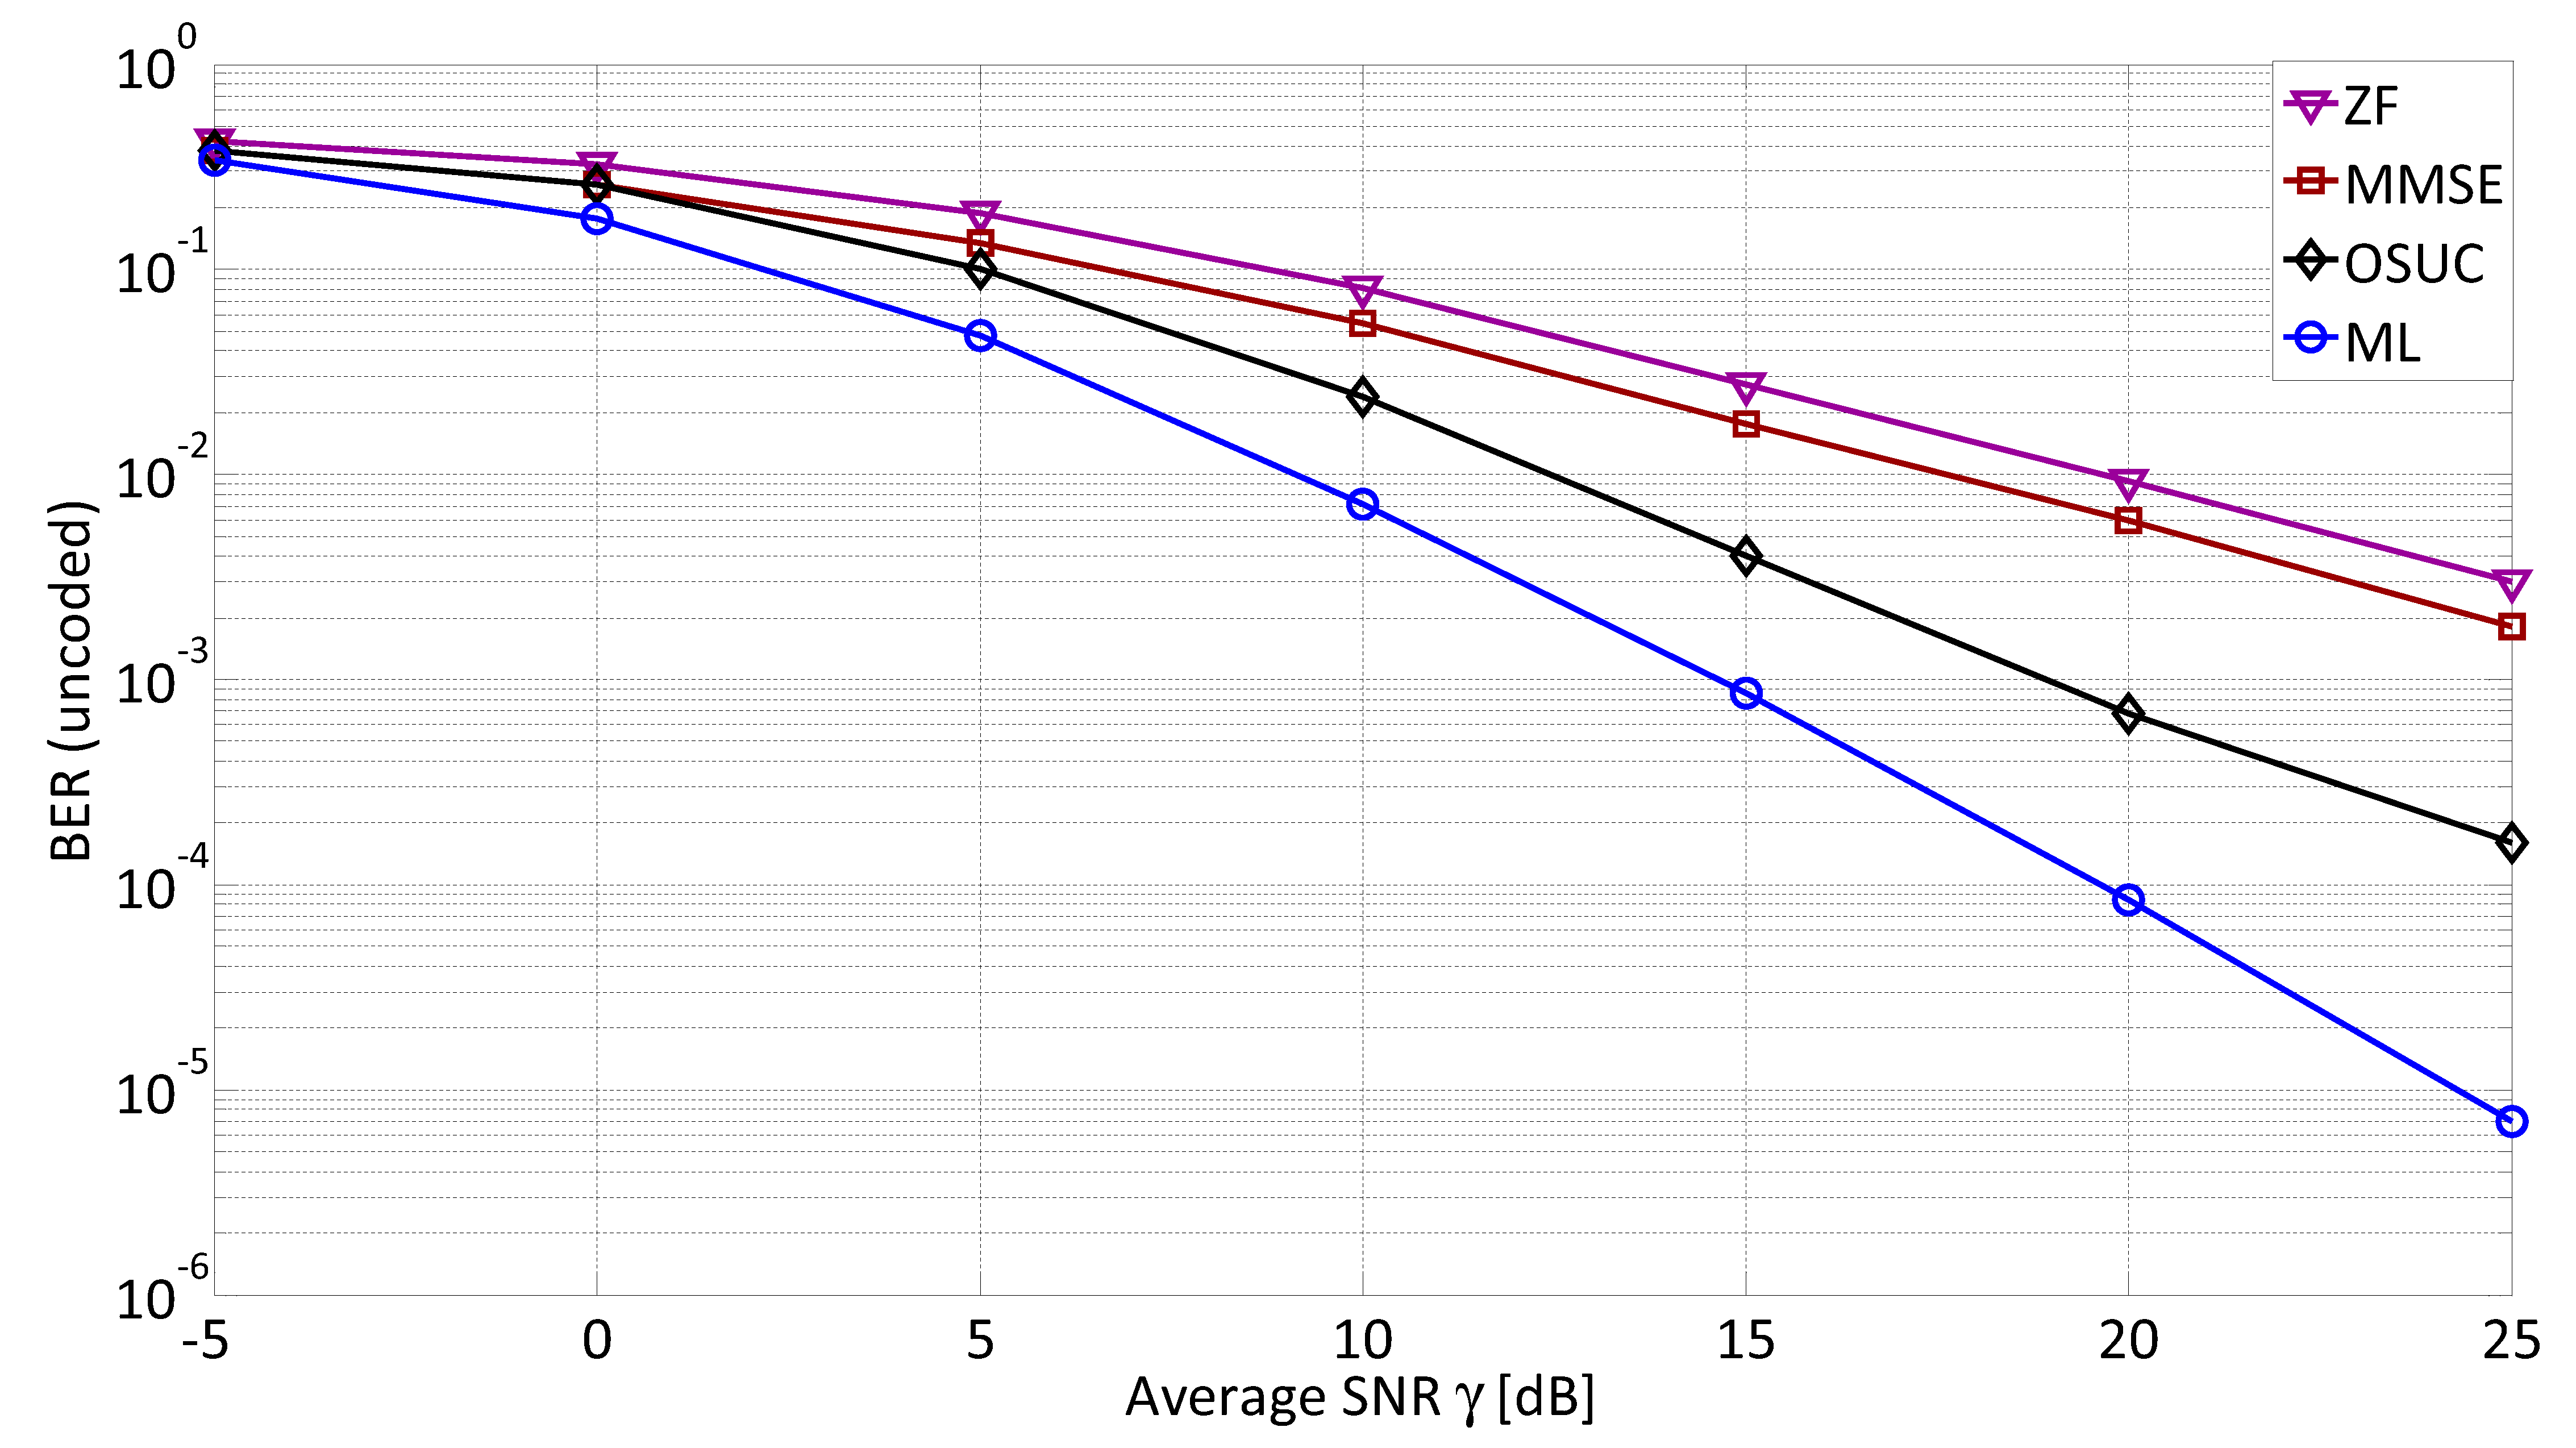
\includegraphics[scale=0.12]{BER_RayleighChannel_ML_MMSE_ZF_OSUC_MODIFIED}

\protect\caption{Bit Error Ratio for two receive antennas receiver in Rayleigh fading
channel in collision slots of two tags\label{fig:Bit-Error-Ratio-ML_MMSE-zf-OSUC}}


\end{figure}



\section{Conclusions}

In this paper, a novel algorithm for decoding two collided and non-synchronized
tags using ML decoding. The algorithm mainly depends on generating
different basis functions instead of regular basis function that are
used when the tags are synchronized. The receiver is tested in a Rayleigh
fading channel with AWGN to see the effect of tolerance on it. The
simulation shows that the tolerance of BLF has no effect on the receiver
performance. The receiver is compared with the ZF, MMSE, and OSUC
receivers that were proposed by \cite{RFID_Reader_Receivers_MIMO}.
The proposed receiver has a diversity gain of order $N_{R}$ while
the MMSE and ZF has a diversity gain of order $1$ and the OSUC has
a diversity gain of order between $1$ and $N_{R}$. The simulation
of the proposed receiver is verified by simulating the other receivers
in the same environment and give the same results of \cite{RFID_Reader_Receivers_MIMO}.


\section*{Acknowledgment}

The authors are grateful to the Fraunhofer IIS for the support of
this work.

\bibliographystyle{IEEEtran}
\bibliography{Refrences}

\end{document}
